All these things are \gap{closely} \gap{related}.
Given one, you can \gap{find} \gap{the} \gap{others}.

\begin{center}  
    \small  
    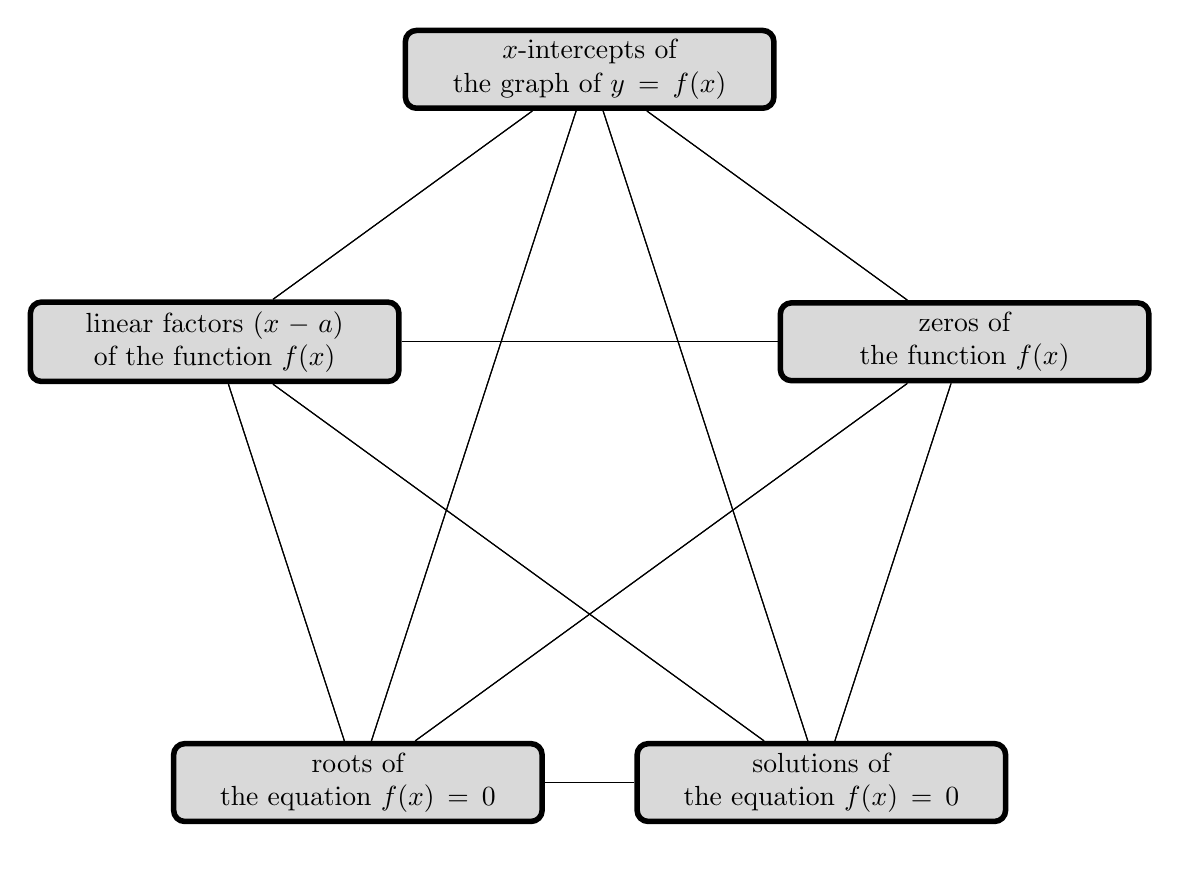
\begin{tikzpicture}
        % Draw a circle around which I'll place nodes.
        \node[circle,minimum size=10cm] (Z) {};
        %
        % Place 5 nodes around the circle.
        \node (rect) [draw,text width=1.75in, align=center,line width=2pt,rounded corners=4pt,fill=black!15] 
            (n-1) at (Z.{90})
            {
                \myEmph{$x$-intercepts} of\linebreak
                the graph of $y=f(x)$
            };
        \node (rect) [draw,text width=1.75in, align=center,line width=2pt,rounded corners=4pt,fill=black!15] 
            (n-2) at (Z.{90+72})
            {
                \myEmph{linear factors} $(x-a)$\linebreak
                of the function $f(x)$
            };
        \node (rect) [draw,text width=1.75in, align=center,line width=2pt,rounded corners=4pt,fill=black!15] 
            (n-3) at (Z.{90+144})
            {
                \myEmph{roots} of\linebreak
                the equation $f(x)=0$
            };
        \node (rect) [draw,text width=1.75in, align=center,line width=2pt,rounded corners=4pt,fill=black!15] 
            (n-4) at (Z.{90+216})
            {
                \myEmph{solutions} of\linebreak
                the equation $f(x)=0$
            };
        \node (rect) [draw,text width=1.75in, align=center,line width=2pt,rounded corners=4pt,fill=black!15] 
            (n-5) at (Z.{90+288})
            {
                \myEmph{zeros} of\linebreak
                the function $f(x)$
            };
        %
        % Connect all the nodes by lines.
        \foreach\x in{1,...,5}{
            \foreach\y in{1,...,5}{
            \ifnum\x=\y\relax\else
                \draw (n-\x) edge[-] (n-\y);
            \fi
            }
        }
    \end{tikzpicture}
\end{center}